\chapter{Introducción}
\label{chapter:introduccion}

\chapquote{Si he logrado ver más lejos ha sido porque he subido a hombros de gigantes.}{Isaac Newton}
\todo[inline]{Quizás toque cambiarla para no repetirse con la intro}

\section{Contexto}


Según la Organización Mundial de la Salud, podemos definir la salud mental como "un estado de bienestar mental que permite a las personas hacer frente a los momentos de estrés de la vida, desarrollar todas sus habilidades, poder aprender y trabajar adecuadamente y contribuir a la mejora de su comunidad" \cite{oms_salud_2022}, siendo parte integral de la salud y el bienestar de una persona; tal y como reflejada en la definición de salud de la OMS: “La salud es un estado de completo bienestar físico, mental y social, y no solamente la ausencia de afecciones o enfermedades” \cite{feafes_galicia_que_nodate}. 

Una vez establecido qué es la salud mental, podemos hablar de su situación actual dentro de nuestra sociedad. Desafortunadamente, este área de la salud ha estado rodeada de una gran estigmatización \cite{delgado_rompiendo_2021}  \cite{andres_tallarda_combatir_2020}, afectada por una gran cantidad de prejuicios hacia las enfermedades y los pacientes que las sufren. En este sentido, según la Fundación de Salud Mental de Inglaterra, nueve de cada diez personas que sufren algún problema de salud mental se han visto afectadas negativamente por el estigma o la discriminación \cite{mental_health_foundation_stigma_nodate}.

Si bien en los últimos años ha ganado visibilidad y atención, gracias a la paulatina concienciación por parte de individuos particulares, o por actores estatales mediante iniciativas como la creación del 
Observatorio Estatal de Salud Mental, Derechos e Igualdad \cite{comunicacion_nace_2022} o su inclusión en los Objetivos de Desarrollo Sostenible \cite{oms_salud_nodate},  las enfermedades relacionadas con la salud mental son un problema de fondo que afecta profundamente a nuestra sociedad, que tradicionalmente no ha gozado de la importancia que merece.

Sus consecuencias y estadísticas, como veremos a continuación, son demoledoras; y que en muchas ocasiones continua siendo un tema tabú. Transciende mucho más allá de "simples" pensamientos de angustia o tristeza, siendo una cuestión que, como sociedad, no estamos siendo capaces de solucionar.

Según el informe "La situación de la Salud Mental en España 2023" \cite{comunicacion_cuatro_2023}, realizado con la colaboración de más de 2.000 personas, el 39,3\% de las personas valoraban de forma negativa su salud mental actual. Asimismo, el 42,1\% han sufrido una depresión a lo largo de su vida, mientras que un 36,9\%, ansiedad prolongada en el tiempo. 

Las duras estadísticas no acaban aquí. Quizás una de los efectos más visibles de los problemas de salud mental sea el suicidio. Desgraciadamente, en España, durante 2022 se suicidaron 4.227 personas, es decir, once vidas perdidas cada día. Una estadística absolutamente demoledora que desde 2018, no para de aumentar (ver figura \ref{fig:intro:muertes_suicidio}).

\begin{figure}[h]
    \centering
    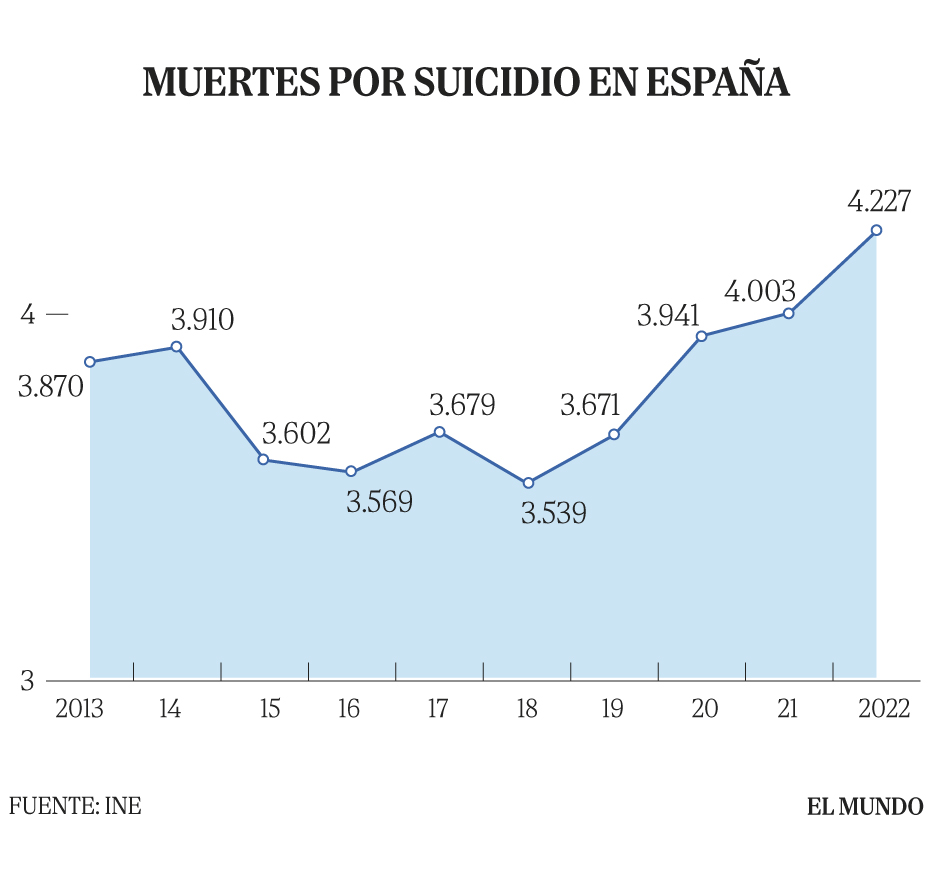
\includegraphics[width=0.66\linewidth]{figures/muertes_suicidio.jpg}
    \caption{Muertes por suicidio en España desde 2013 hasta 2022 \cite{saiz_4227_2023}}
    \label{fig:intro:muertes_suicidio}
\end{figure}

Asimismo, el suicidio se mantiene como primera causa no natural de muerte en nuestro país desde 2008, por encima de otras quizá más presentes en el imaginario colectivo, como los accidentes de tráfico o los ahogamientos (ver figura \ref{fig:intro:causas_no_naturales}).

\begin{figure}[h]
    \centering
    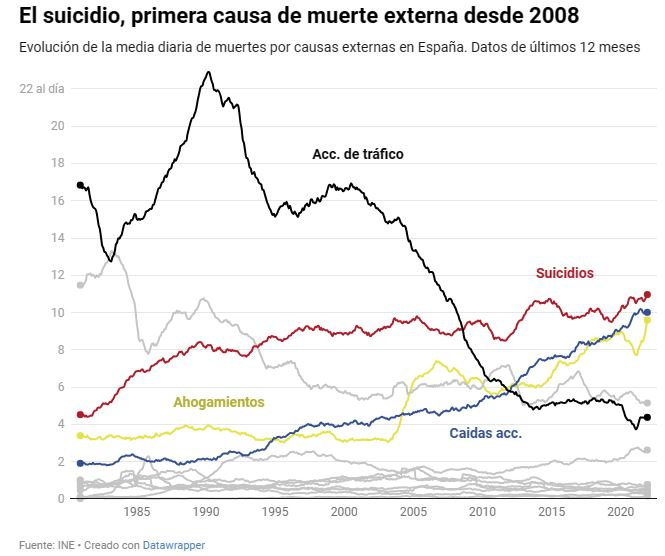
\includegraphics[width=0.85\linewidth]{figures/causas no naturales.jpg}
    \caption{Evolución de la media diaria de las muertes por causas no naturales en España, desde 1980 a 2021 \cite{sanchez_once_2023}}
    \label{fig:intro:causas_no_naturales}
\end{figure}

No obstante, esta funesta métrica solo muestra a las personas que desgraciadamente decidieron acabar con su vida, sin mostrar los casos de personas que sufren en vida. Sin ir más lejos, según el catedrático en Psiquiatría Jose Luis Ayuso Mateos "por cada persona que fallece, hay 25 que lo han intentado"  \cite{sanchez_once_2023}.  Por otra parte el 14,5\% de la población ha tenido ideas suicidas o lo ha intentado \cite{comunicacion_cuatro_2023}.

Detrás de las estadísticas, podemos encontrar testimonios de familiares que quedaron rotos tras el suicidio de un ser querido. De lo profundamente cruel e invisible que puede ser una enfermedad mental. Asimismo, otra problemática que presentan enfermedades como la depresión es su invisibilidad. Según datos de la asociación La Barandilla, el 30\% de las personas que padecen depresión no lo hablan con su familia \cite{abc_familia_30_2021}.

Enfermedades como la depresión es un factor que puede conducir a una persona a suicidarse. En las redes sociales podemos encontrar duros y crudos testimonios de familiares a los que la depresión arrebató de sus vidas a un ser querido, los cuales transcienden de las estadísticas, tal y como se puede ver en la figura \ref{fig:intro_testimonio_madre} .

\begin{figure}[h]
    \begin{subfigure}[b]{0.49\textwidth}
        
\includegraphics[width=1\linewidth]{figures/testimonio_madre_1.jpg}
    \end{subfigure}
    \hfill
    \begin{subfigure}[b]{0.49\textwidth}
        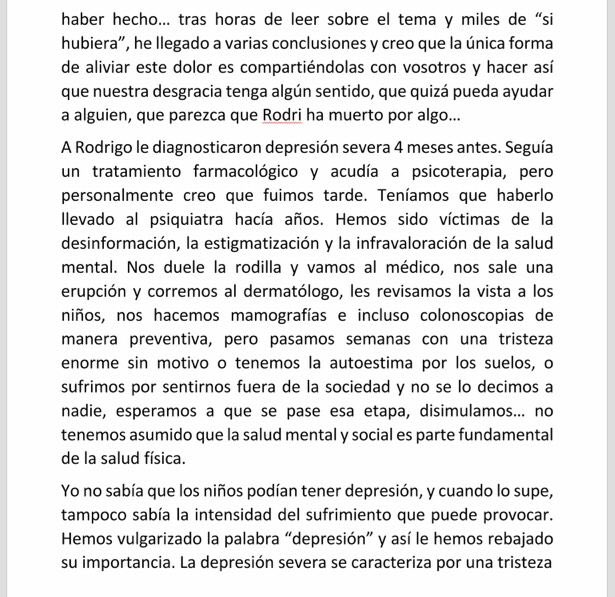
\includegraphics[width=1\linewidth]{figures/testimonio_madre_2.jpg}
    \end{subfigure}
    \caption{Extracto del testimonio de una madre tras el suicidio de su hijo \cite{irene_pujol_i_athenea_hace_2021}}
    \label{fig:intro_testimonio_madre}
\end{figure}

Por otra parte, las enfermedades mentales afectan a todo tipo de personas. Algunas personas que podríamos considerar como exitosas han sufrido problemas de salud mental, desde "pequeños" brotes como Alejandro Sanz \cite{lopez_chicon_que_2023} \cite{riano_alejandro_2023}, hasta casos de suicidio, como el del cantante Chester Bennington, famoso vocalista del grupo Linkin Park, el cual experimentó depresión durante largas fases de su vida \cite{el_universal_nada_2020} \cite{gambin_historia_2022}.

Una vez visto el impacto de las enfermedades mentales en nuestra sociedad, podemos preguntarnos cómo se puede relacionar la Informática con la Salud Mental. El uso de redes sociales podría afectar a nuestra salud mental \cite{burn-murdoch_smartphones_2023}, siendo un tema de debate en la Academia. Algunos argumentos que ratificarían esa afirmación son un espectacular incremento de los ratios de suicidio en jóvenes desde la popularización de los smartphones y redes sociales en Estados Unidos como en Reino Unido, o la multiplicación por 4 de los ratios de depresión en Francia entre las personas de 15 a 24 años en la última década.

Por otra parte, la popularización de los smartphones y de los \textit{wearables} permite obtener más información sobre el comportamiento de la persona (uso del móvil, ejercicio físico, hábitos de sueño), sus constantes vitales (pulsaciones, niveles de oxígeno en sangre), lo que podría ayudar a la detección precoz de problemas de salud mental.

\todo[inline]{Pensar si esto aqui o en la justificación}


\section{Objetivos}

    \subsection{Objetivo general}
    El objetivo principal del proyecto es la creación del prototipo de un Sistema para el Bienestar Emocional, mediante la detección precoz y mejora de los trastornos de salud mental en la comunidad universitaria (estudiantes, profesores y personal de administración y servicios). 
    
    Para ello, el sistema contará con dos partes principales: una aplicación Android y un conjunto de dispositivos hardware \textit{wearables}. Estos últimos serán los encargados de recoger datos físicos del usuario, tales como frecuencia cardíaca, hábitos de sueño, distancia recorrida, ejercicio físico realizado...
    
    Por otra parte, la aplicación obtendrá dichos datos para proporcionar al usuario detalles de su estado de bienestar y en base a ellos, proporcionar ejercicios, medidas de autocontrol, sugerencias e incluso orientaciones para buscar la asesoría médica y profesional en caso de ser necesario.

Dado que este proyecto es un prototipo de un escenario de uso concreto, éste puede ser extendido no solo a diferentes escenarios, sino que, a futuro, con los datos recogidos y anonimizados se podría
desarrollar y entrenamiento de un módulo para ayudar en la detección precoz de trastornos asociados a la salud mental como el nivel de estrés de los usuarios.

    \subsection{Objetivos específicos}
    Para completar el objetivo general, los siguientes objetivos específicos han sido establecidos:
    \begin{itemize}
        \item Uso de metodologías y estándares propios de la Ingeniería de Sistemas para la extracción de requisitos y diseño. En particular se utilizarán los estándares IEEE 830 y SysML, respectivamente.
        \item Implementación de la aplicación Android con las tecnologías recomendadas para los nuevos desarrollos. 
        \item Lectura de datos de los \textit{wearables} mediante componentes software reutilizables. Para ello se deberá estudiar qué posibilidades existen para el acceso a los datos y la compatibilidad con las pulseras disponibles en el mercado español.
        \item Diseño e implementación de una interfaz gráfica de calidad, agradable para el usuario. Con esto se pretende una experiencia de uso cómoda para el usuario, especialmente en el uso de la aplicación y la visualización de los datos. 
        \item Como muestras de calidad, la aplicación Android deberá ser \textit{responsive}, para que se adaptarte a las diferentes pantallas de los usuarios, mientras que los textos de la aplicación deberán estar disponibles tanto en castellano como en inglés para permitir el uso por parte de cualquier persona de la comunidad universitaria.
    \end{itemize}

\section{Motivación}

Este proyecto no nace de una situación concreta o definida, o de una lista de temas propuestos, sino principalmente del impacto que ha tenido la salud mental en mi vida, tanto a nivel propio como en personas cercanas. El pertenecer a otra área del conocimiento, alejada de las Ciencias de la Salud, supone al mismo tiempo una desventaja como una posibilidad de aportar desde un prisma completamente diferente, permitiendo la colaboración con personas de diferente formación y ocupación.

Desde un punto de vista más informático, los aspectos que han motivado la realización de este proyecto son las siguientes:
\begin{itemize}
    \item Creación de una app Android completa con las nuevas herramientas de las que dispone el \textit{framework}, para crear aplicaciones más completas y más rápidamente.
    \item Exploración del \textit{framework} Health Connect, tanto para la escritura de datos (desde el punto de vista de los \textit{wearables}) como la lectura de los mismos (desde la aplicación Android).
    \item 
    \item Interconexión de una aplicación móvil con un servidor
\end{itemize}

Asimismo, otra vertiente del proyecto radica en la exploración de las posibilidades que ofrecen los \textit{wearables} tanto para desarrolladores como científicos.


. La selección de este tema en particular obedece a una serie de circunstancias personales que, tras años pululando por los rincones de mi mente, tomaron esta forma.

La motifa

En primer lugar, mi motivación principal es el deseo de querer hacer algo para ayudar, aunque sea modestamente, a la mejora de la salud mental dentro de nuestra sociedad. Para bien o para mal, en mi vida he estado expuesto a la importancia de la salud mental. En ocasiones he podido ver a personas que se sienten realizadas y felices con situaciones que, a los ojos de terceras personas, quizás no sean precisamente ideales; pero por otra parte he sentido impotencia y dolor al ver cómo la depresión u otras enfermedades destruyen la vida de un ser querido. También he vivido incertidumbre y pánico cuando ves que hay algo dentro de ti que no está bien y que no sabes ni por qué, ni cómo resolver. Son situaciones cuanto menos, impactantes.

Desafortunadamente, como sociedad no somos capaces en muchas ocasiones de dar una respuesta, una solución a esas problemáticas. Es una cuestión bastante amplia que necesita esfuerzos desde múltiples sectores de la sociedad, y ahí puede contribuir con su granito de arena la Informática.

Como se suele decir, el primer paso para resolver un problema es reconocerlo. La Salud Mental ha sido ignorada, subestimada... poco menos que maltratada. Si bien no deja de ser algo subjetivo y particular, tengo la percepción de que en muchas ocasiones se trata de puro desconocimiento, de no entender un problema de salud que no se ve a simple vista. De entender algo que se había relegado al ostracismo, a la estigmatización. 

Por tanto, este TFM está dirigido a visibilizar la Salud Mental, a través de los siguientes factores:

\begin{itemize}
    \item 
\end{itemize}


Esa impotencia que sientes cuando ves a alguien cercano sufrir y no tener idea de cómo ayudar. También esa  Esas fuerzas son suficientes para motivarte de, cuando sea posible, intentar tomar cartas en este asunto. Quizás no ya para ayudar a alguien próximo, sino para intentar reducir el número de personas que puedan sentirlo alguna vez. 

Como mis estudios están alejados de esas ciencias, 


, sino de un conjunto de vivencias personalmente. La Salud Mental es algo que, a pesar de que gran parte de la sociedad no quiera ver, está ahí, tanto para lo bueno o para lo malo. Ver de primera mano cómo una depresión puede condicionar la vida de un ser querido y sentir impotencia por no poder ayudar, sentir en tus propias carnes como a veces no te encuentras bien y no sabes por qué... es motivación suficiente como para interesarte por este tema.

Solo escribir la introducción ya te pone el corazón en un puño.

Si bien la Informática puede verse como un área alejada de la Salud Mental, se puede realizar una contribución hacia la misma

\section{Justificación}

Las estadísticas sobre la salud mental arrojan una preocupante tendencia de cara al futuro, tanto a nivel nacional como internacional. Según estadísticas de la Confederación Salud Mental España \cite{confederacion_salud_mental_espana_salud_nodate} \cite{aguilar_laura_2022},  en España más de la mitad de las de las personas con trastorno mental que necesitan tratamiento no lo reciben, y un porcentaje significativo no recibe el adecuado. 

Asimismo, dentro de la atención médica, en España solo se disponen en la Sanidad Pública de seis psicólogos por cada 100.000 habitantes en la red pública \cite{antolin_listas_2023}, muy por debajo de países de nuestro entorno como Alemania (41), Reino Unido (18) o Francia (15), entre otros. 

Las listas de espera dentro de la sanidad pública, frecuentemente constando de meses según las poca información suministrada por las CC.AA. \cite{asuar_gallego_recurrir_2021} \cite{pascual_listas_2021}, hacen que la salud mental sea poco menos que un lujo, sin entrar a la valorar la calidad de la misma. Para el 57,3\% de la población  \cite{comunicacion_cuatro_2023}, acudir a un profesional de la salud mental privado es algo económicamente inaccesible.

\begin{figure}[h]
    \centering
    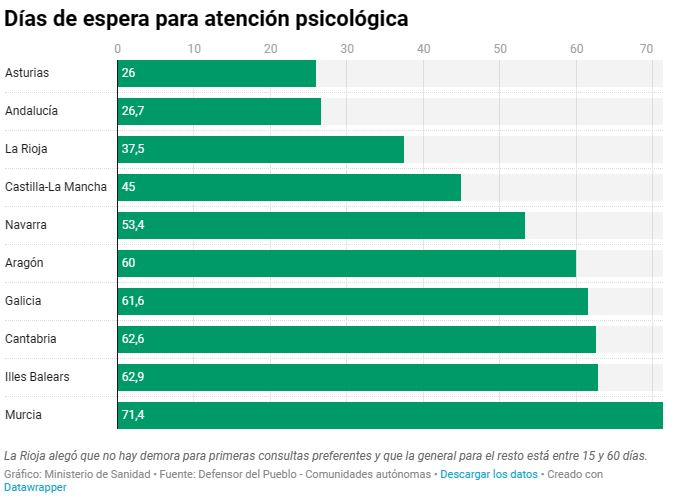
\includegraphics[width=1\linewidth]{figures/dias espera.JPG}
    \caption{Dias de espera para atención psicológica según Comunidades Autónomas \cite{asuar_gallego_recurrir_2021}}
    \label{fig:intro:dias_espera}
\end{figure}

Por otra parte, se estima a nivel mundial una de cada cuatro personas tendrán un trastorno mental a lo largo de su vida, mientras que en España, casi la mitad de los y las jóvenes de entre 15 y 29 años (48,9\%) considera que ha tenido algún problema de salud mental.

\todo[inline]{por que la depresion es jodida y frecuente}
Dentro de estas enfermedades, una de las más conocidX es la depresión.

\todo[inline]{por que la soledad es jodida y frecuente}

No obstante, para la depresión hay condicionantes como la soledad. (Suicidio como efecto, no causa) \href{https://www.sabervivirtv.com/medicina-general/soledad-multiplica-riesgo-depresion_6528}{Por qué la soledad multiplica por 5 el riesgo de depresión (sabervivirtv.com)} 

\todo[inline]{por que el estres es jodida y frecuente}

Estos datos ponen de manifiesto la necesidad crítica de trabajar tanto en la prevención, en el diagnóstico precoz y en la atención a las personas que sufren un trastorno mental que, bien por desconocimiento o por estigma, no reciben el tratamiento que necesitan.

En esta necesidad fehaciente se sitúan numerosas iniciativas, como "Special Initiative for Mental Health (2019-2023)" \cite{oms_salud_nodate} de la OMS, o dentro de España, la "Estrategia de Salud Mental" o la línea 024 de atención a la conducta suicida \cite{la_moncloa_minones_2023}.

\section{Estructura del documento}

En este documento se detalla paso a paso el proceso que se ha seguido para el desarrollo del proyecto, partiendo desde el análisis, continuando por el diseño y finalizando en la implementación y pruebas. 

En particular, la memoria consta de la siguiente estructura:
\begin{enumerate}
    \item Introducción
    \item Marco teórico
    \item Estado del arte
    \item Metodología 
    \item Análisis del sistema
    \item Diseño de la solución
    \item Implementación del sistema
    \item Pruebas del sistema
    \item Resultados obtenidos
    \item Impacto social y medioambiental
    \item Presupuesto
    \item Conclusiones
    \item Líneas futuras
\end{enumerate}